\chapter*{Error yang biasa ditemukan saat melakukan sintak}
\section*{Error dalam menggunakan tanda kurung}
\begin{enumerate}
	\item dalam melakukan sintak print terkadang kita lupa untuk memberi tanda kurung sehingga sintak error
	\begin{figure} [h]
	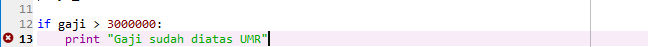
\includegraphics[width=12cm]{error/er1.png}
	\centering
	\end{figure}
	
    \item seharusnya ditulis seperti berikut
	\begin{figure} [h]
	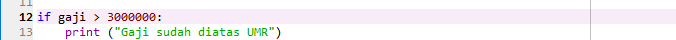
\includegraphics[width=12cm]{error/er2.png}
	\centering
	\end{figure}

\section*{Error penulisan huruf besar pada kondisi}
	
	
	\item Terkadang kita juga lupa untuk menggunakan huruf besar saat melakukan sintak kondisi 
	\begin{figure} [h]
	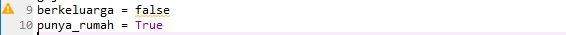
\includegraphics[width=9cm]{error/er3.png}
	\centering
	\end{figure}
	
	\item Seharusnya dituliskan sebagai berikut 
	\begin{figure} [h]
	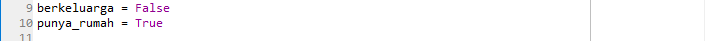
\includegraphics[width=9cm]{error/er4.png}
	\centering
	\end{figure}
	
	
\end{enumerate}